\documentclass[14pt]{beamer}

\usepackage[czech]{babel}				% Jazyk
\usepackage[a-2u]{pdfx}					% Kopírování z pdfka
\usepackage{tikz}						% Schémata automatů
\usepackage{csquotes}					% české uvozovky
\usepackage{enumerate}					% enumerate environment
\usepackage{indentfirst}
\usepackage{mathtools}
\usepackage{pifont}
\usepackage{xcolor}
\usepackage{enumitem,xcolor}
\usepackage{amsmath}
\usepackage[utf8]{inputenc}

\usepackage{listings}                   % Úryvky z kódu (C#)
\lstset{language=[Sharp]C, frame=lr}

% Assets
% Beamer theme
\usetheme{Boadilla}
\setbeamertemplate{frame numbering}[fraction]
\usecolortheme[named=black]{structure}
\setbeamertemplate{navigation symbols}{}
\setbeamerfont{title}{series=\bfseries,parent=structure}
\setbeamerfont{frametitle}{series=\bfseries,parent=structure}
\usefonttheme[onlymath]{serif}
\urlstyle{same}

% Dark theme
\setbeamercolor{frametitle}{fg=white}
\setbeamercolor{title}{fg=white}
\setbeamercolor{background canvas}{bg=black}
\setbeamercolor{normal text}{fg=white}

\defbeamertemplate*{title page}{customized}[1][]
{ 
  \usebeamerfont*{title}\inserttitle\par
  \bigskip
  \usebeamerfont*{subtitle}\textit{\insertsubtitle}\par
  \bigskip \bigskip \bigskip \bigskip 
  \usebeamerfont{author}\insertauthor\par
  \usebeamerfont{institute}Kabinet \office\\\url{weber3@spsejecna.cz}\bigskip
}
% Enumerate
%\setlist[enumerate]{topsep=0pt,itemsep=-1ex,partopsep=1ex,parsep=1ex,label=(\arabic*)}

\MakeOuterQuote{"}

% Colors
\definecolor{lightblue}{HTML}{009AD4}
\definecolor{darkgreen}{HTML}{0D7103}
\definecolor{lightgreen}{HTML}{68FF00}
\definecolor{darkred}{HTML}{AF0B0B}
\definecolor{lightred}{HTML}{FF5100}
\definecolor{orange}{HTML}{FFE000}
\definecolor{codeblue}{HTML}{FF0055}
\definecolor{codegreen}{rgb}{0,0.6,0}
\definecolor{codegray}{rgb}{0.5,0.5,0.5}
\definecolor{codebeige}{HTML}{D4A000}
\definecolor{backcolour}{rgb}{0.95,0.95,0.92}

\newcommand{\markred}[1]{\textcolor{lightred}{#1}}
\newcommand{\markgreen}[1]{\textcolor{lightgreen}{#1}}
\newcommand{\markorange}[1]{\textcolor{orange}{#1}}
\newcommand{\markblue}[1]{\textcolor{lightblue}{#1}}

% Inline images
\newcommand{\inlineimgscale}{1.1}

% X and check mark
\newcommand{\cmark}{\markgreen{\ding{51}}}
\newcommand{\xmark}{\markred{\ding{55}}}

% Redefinions
\renewcommand{\implies}{\Rightarrow}
\renewcommand{\impliedby}{\Leftarrow}

% Math
\newcommand{\R}{\mathbb{R}}
\newcommand{\C}{\mathbb{C}}
\newcommand{\N}{\mathbb{N}}
\newcommand{\Z}{\mathbb{Z}}
\newcommand{\Q}{\mathbb{Q}}

% Code
\lstdefinestyle{clang}{
    basicstyle=\small\ttfamily\color{white},
    language=C,
    keywordstyle=\color{codeblue},
    commentstyle=\color{codegreen},
    numberstyle=\tiny\color{codegray},
    stringstyle=\color{codebeige},
    breakatwhitespace=false,
    breaklines=true,
    captionpos=b,
    keepspaces=true,
    numbersep=5pt,
    showspaces=false,
    showstringspaces=false,
    showtabs=false,
    morekeywords={void,int,double,float,unsigned,if,else,\#include}
    tabsize=0.5
}
\lstset{escapeinside={(*}{*)},style=clang}

\newcommand{\hlcode}[1]{\colorbox{red}{#1}}

% Title page
\title{Číselné soustavy}
\author{David Weber}
\date{\today}

\begin{document}

    % Itemize
    \setlist[itemize]{label=\textcolor{white}{\textbullet}}

    % Slides
    \begin{frame}[t]
        \titlepage
    \end{frame}

    \begin{frame}[t]{Nejdříve zopáčko\dots}
        \only<1->{Co rozumíme pod zápisem čísla 963?}
        \only<2->{\begin{align*}
            \only<2->{&\implies\;\text{9 stovek, 6 desítek, 3 jednotky}}\\
            \only<3->{&\implies\;\underbrace{9\cdot 10^2}_{\text{stovky}} + \underbrace{6\cdot 10^1}_{\text{desítky}} + \underbrace{3\cdot 10^0}_{\text{jednotky}}.}
        \end{align*}}
        \only<4->{Pro každý z řádů máme deset symbolů: 0,\,1,\,2,\,\dots,\,9 $\implies$ odtud \textbf{desítková (dekadická) soustava}.}
    \end{frame}

    \begin{frame}[t]{Nejdříve zopáčko\dots}
        \only<1->{Překročíme-li řád, pak zvýšíme hodnotu následujícího a aktuální vynulujeme.}
        \only<2->{\begin{align*}
            \dots &000\, 1\\
            \dots &000\, 2\\
            &\vdots\\
            \dots &000\, 9\\
            \dots &001\, 0 \leftarrow\text{Vynulujeme a zvýšíme řád desítek}
        \end{align*}}
    \end{frame}

    \begin{frame}[t]{Nejdříve zopáčko\dots}
        \only<1->{Co kdybychom měli např. pouze 5 číslic na řád, tzn. 0,\,1,\,2,\,3,\,4?}
        \only<2->{\begin{center}
            \markgreen{Princip bude zcela stejný. :-)}
        \end{center}}
        \only<3->{\begin{itemize}
            \only<3->{\item \markorange{$\implies$ Řády nyní interpretujeme v mocninách \textbf{pětky}!}}
            \only<4->{\item Číslo 5 zde představuje tzv. \textbf{základ soustavy}.}
            \only<5->{\item Např. $4233_5$ tak bude rovno
            \begin{equation*}
                \boxed{4}\cdot 5^3+\boxed{2}\cdot 5^2+\boxed{3}\cdot 5^1+\boxed{3}\cdot 5^0=568
            \end{equation*}
            v desítkové soustavě.}
        \end{itemize}}
    \end{frame}

    \begin{frame}[t]{Totéž obecněji}
        \begin{itemize}
            \item Mějme nějakou soustavu o základu $Z$ (tzn. máme celkem $Z$ symbolů na řád).
            \item Libovolné číslo $(a_na_{n-1}a_{n-2}\dots a_0)_Z$ má pak hodnotu
            \begin{equation*}
                a_n\cdot Z^n+a_{n-1}\cdot Z^{n-1}+\cdots +a_1\cdot Z^1 + a_0\cdot Z^0\,,
            \end{equation*} 
            kde koeficienty $a_i$ jsou menší než základ $Z$.
        \end{itemize}
    \end{frame}

    \begin{frame}[t]{Významné soustavy}
        \only<1->{\begin{itemize}
            \only<1->{\item \markgreen{Desítková}}
            \only<2->{\item \markorange{Dvojková (binární)}
            \begin{itemize}
                \item Pouze číslice 0 a 1.
            \end{itemize}}
            \only<3->{\item \markorange{Šestnáctková (hexadecimální)}
            \begin{itemize}
                \item 16 symbolů na řád.
            \end{itemize}}
        \end{itemize}}
    \end{frame}

    \begin{frame}[t]{Dvojková soustava}
        \only<1->{\begin{itemize}
            \only<1->{\item Též \textbf{binární} soustava.}
            \only<2->{\item Pouze číslice 0 a 1 $\implies$ řád soustavy je 2.}
            \only<3->{\item Např. číslo $110001_2$ je v desítkové soustavě
            \begin{align*}
                &\boxed{1}\cdot 2^5+\boxed{1}\cdot 2^4+\boxed{0}\cdot 2^3+\boxed{0}\cdot 2^2+\boxed{0}\cdot 2^1+\boxed{1}\cdot 2^0\\
                &=32+16+0+0+0+1\\
                &=49.
            \end{align*}}
            \only<4->{\item Využívána v počítačích (elektrické obvody) $\implies$ dva jednoduše rozlišitelné stavy (zapnuto/vypnuto).}
        \end{itemize}}
    \end{frame}

    \begin{frame}[t]{Šestnáctková soustava}
        \only<1->{\begin{itemize}
            \item Též \textbf{hexadecimální} soustava.
            \item 16 symbolů na řád.
            \begin{itemize}
                \item Číslice $0,\,1,\,\dots,\,9$ a
                \item písmena $A,\,B,\,\dots,\,F$ $\leftarrow$ chápeme jako hodnoty $10,\,11,\,\dots,\,15$.
            \end{itemize}
        \end{itemize}}
        \only<2->{\begin{align*}
            \text{FA8B}_{16}&=\overbrace{\boxed{15}}^{\text{F}}\cdot 16^3+\overbrace{\boxed{10}}^{\text{A}}\cdot 16^2+\boxed{8}\cdot 16^1+\overbrace{\boxed{11}}^{\text{B}}\cdot 16^0\\
            &=61440+2560+128+11\\
            &=64139.
        \end{align*}}
    \end{frame}

    \begin{frame}[t]{Šestnáctková soustava}
        \only<1->{Proč zrovna základ 16?}
        \only<2->{\begin{itemize}
            \only<2->{\item Dvojková soustava není vždy vhodná pro zápis větších čísel.}
            \only<3->{\item Např. číslo 3834 je binárně $111011111010_2$.\\
            \markred{$\implies$ potřebujeme 12 symbolů pro zápis!}}
            \only<4->{\item V hexadecimálním zápisu $3834=\text{EFA}_{16}$ nám stačí\\\markgreen{3 symboly}.}
            \only<5->{\item Lze elegantně využít faktu, že $16=2^4$.}
        \end{itemize}}
    \end{frame}

    \begin{frame}[t]{Šestnáctková soustava}
        \only<1-4>{Rozepišme si číslo 3834:}
        \only<2-4>{\begin{align*}
            3834&=111011111010_2\\
            &=\boxed{1}\cdot 2^{11}+\boxed{1}\cdot 2^{10}+\boxed{1}\cdot 2^9+\boxed{0}\cdot 2^8+\\
            &+\boxed{1}\cdot 2^7+\boxed{1}\cdot 2^6+\boxed{1}\cdot 2^5+\boxed{1}\cdot 2^4+\\
            &+\boxed{1}\cdot 2^3+\boxed{0}\cdot 2^2+\boxed{1}\cdot 2^1+\boxed{0}\cdot 2^0.
        \end{align*}}
        \only<3-4>{Z každé čtveřice sousedních členů vytkneme nejnižší mocninu dvojky:}
        \only<5-7>{Každý z koeficientů před závorkami lze nahradit mocninou čísla $16=2^4$:}
        \only<8->{Výrazy v závorkách jsou rovny $13$, $15$ a $10$ a odpovídají jednotlivým čtveřicím číslic původního čísla.}
        \only<4-5>{\begin{align*}
            3834&=2^8\cdot(1\cdot 2^3+1\cdot 2^2+1\cdot 2^1+0\cdot 2^0)+\\
            &+2^4\cdot(1\cdot 2^3+1\cdot 2^2+1\cdot 2^1+1\cdot 2^0)+\\
            &+2^0\cdot(1\cdot 2^3+0\cdot 2^2+1\cdot 2^1+0\cdot 2^0).
        \end{align*}}
        \only<6>{\begin{align*}
            3834&=(2^4)^2\cdot(1\cdot 2^3+1\cdot 2^2+1\cdot 2^1+0\cdot 2^0)+\\
            &+(2^4)^1\cdot(1\cdot 2^3+1\cdot 2^2+1\cdot 2^1+1\cdot 2^0)+\\
            &+(2^4)^0\cdot(1\cdot 2^3+0\cdot 2^2+1\cdot 2^1+0\cdot 2^0).
        \end{align*}}
        \only<7>{\begin{align*}
            3834&=16^2\cdot(1\cdot 2^3+1\cdot 2^2+1\cdot 2^1+0\cdot 2^0)+\\
            &+16^1\cdot(1\cdot 2^3+1\cdot 2^2+1\cdot 2^1+1\cdot 2^0)+\\
            &+16^0\cdot(1\cdot 2^3+0\cdot 2^2+1\cdot 2^1+0\cdot 2^0).
        \end{align*}}
        \only<8->{\begin{align*}
            3834&=16^2\cdot(\overbrace{1\cdot 2^3+1\cdot 2^2+1\cdot 2^1+0\cdot 2^0}^{\implies\markgreen{1110_2}})+\\
            &+16^1\cdot(\overbrace{1\cdot 2^3+1\cdot 2^2+1\cdot 2^1+1\cdot 2^0}^{\implies\markgreen{1111_2}})+\\
            &+16^0\cdot(\overbrace{1\cdot 2^3+0\cdot 2^2+1\cdot 2^1+0\cdot 2^0}^{\implies\markgreen{1010_2}}).
        \end{align*}}
        \only<9>{\begin{equation*}
            \boxed{1110}\;\boxed{1111}\;\boxed{1010}
        \end{equation*}}
        \only<10>{\begin{equation*}
            \underbrace{\boxed{1110}}_{13=\markgreen{\text{E}_{16}}}\underbrace{\boxed{1111}}_{15=\markgreen{\text{F}_{16}}}\underbrace{\boxed{1010}}_{10=\markgreen{\text{A}_{16}}}
        \end{equation*}}
        \only<11>{\begin{equation*}
            \underbrace{\boxed{1110}}_{13=\text{E}_{16}}\underbrace{\boxed{1111}}_{15=\text{F}_{16}}\underbrace{\boxed{1010}}_{10=\text{A}_{16}}\markgreen{\implies\text{EFA}_{16}}
        \end{equation*}}
    \end{frame}

    \begin{frame}[t]{Šestnáctková soustava}
        \only<1->{\begin{itemize}
            \only<1->{\item Číslo \textbf{z binární do šestnáctkové soustavy} lze převést tak, že převedeme jednotlivé čtveřice číslic jeho binárního zápisu (od nejnižšího řádu).}
            \only<2->{\item Např. převedeme číslo $1000111101_2$ do šestnáctkové soustavy:}
            \only<3>{\begin{equation*}
                1000111101
            \end{equation*}}
            \only<4>{\begin{equation*}
                10\,|\,0011\,|\,1101
            \end{equation*}}
            \only<5>{\begin{equation*}
                \overbrace{\markorange{00}}^{\mathclap{\text{Doplním na čtveřici}}}10\,|\,0011\,|\,1101
            \end{equation*}}
            \only<6>{\begin{equation*}
                0010\,|\,0011\,|\,1101
            \end{equation*}}
            \only<7>{\begin{equation*}
                \underbrace{0010}_{2=2_{16}}\,|\,\overbrace{0011}^{3=3_{16}}\,|\,\underbrace{1101}_{13=\text{D}_{16}}
            \end{equation*}}
            \only<8>{\begin{equation*}
                \underbrace{0010}_{2=2_{16}}\,|\,\overbrace{0011}^{3=3_{16}}\,|\,\underbrace{1101}_{13=\text{D}_{16}}\markgreen{\implies\text{23D}_{16}}
            \end{equation*}}
        \end{itemize}}
    \end{frame}

    \begin{frame}[t]{Převody mezi soustavami}
        \only<1>{\begin{figure}[H]
            \centering
            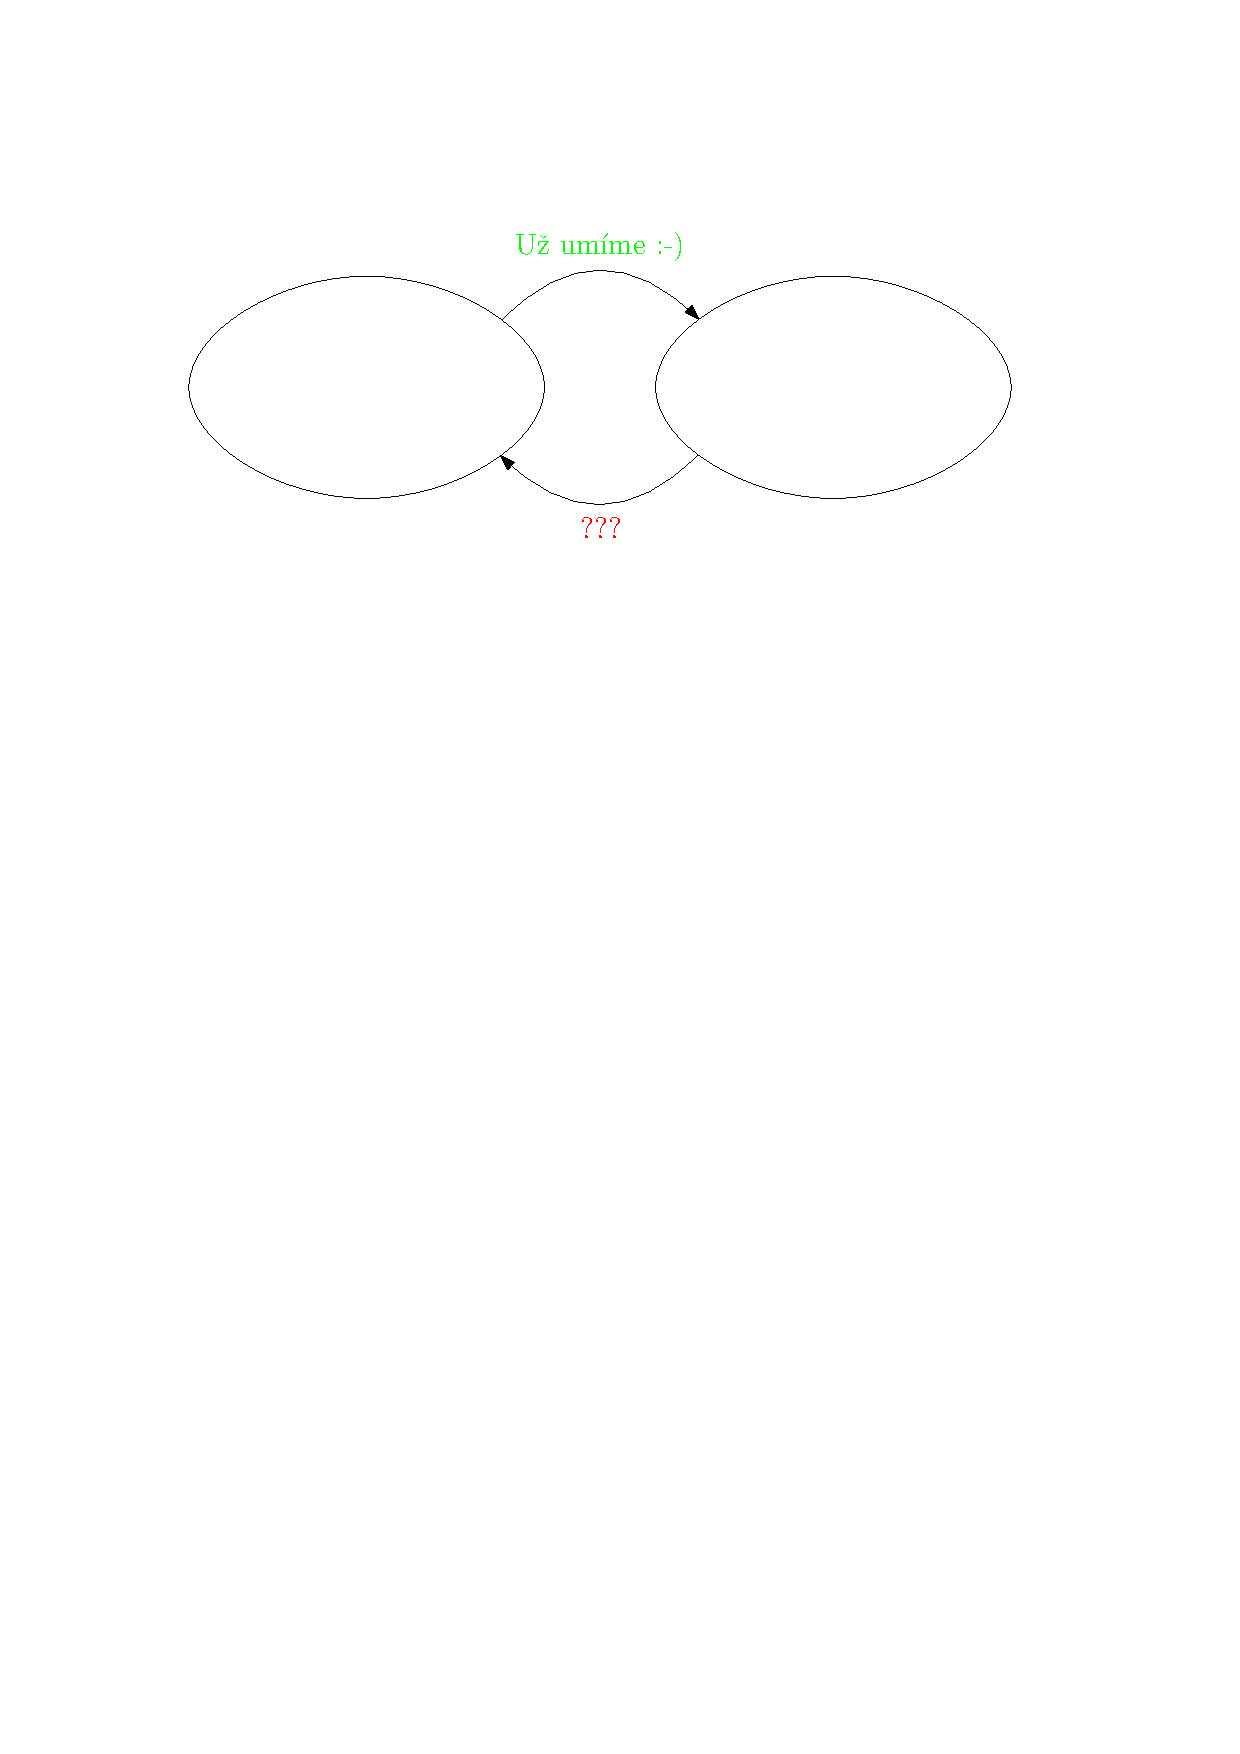
\includegraphics[scale=.7]{images/prevody.pdf}
        \end{figure}}
        \only<2-6>{\begin{itemize}
            \only<2-4>{\item Máme nějaké číslo $x$ v desítkové soustavě}
            \only<3-4>{\begin{center}
                \markorange{$\implies$ chceme vyjádření v soustavě o základu $Z$.}
            \end{center}}
            \only<4-6>{\item Hledáme koeficienty $a_0,\,a_1,\,\dots,\,a_n$, tak, aby platilo
            \begin{align*}
                x&=a_n\cdot Z^n+a_{n-1}\cdot Z^{n-1}+\cdots +a_1\cdot Z^1+a_0\cdot Z^0\\
                &=a_n\cdot Z^n+a_{n-1}\cdot Z^{n-1}+\cdots +a_1\cdot Z^1+a_0
            \end{align*}}
        \end{itemize}}
        \only<5-6>{Až na poslední člen s $a_0$ můžeme všude vytknout základ $Z$:}
        \only<6-10>{\begin{align*}
            (a_n\cdot Z^{n-1}+a_{n-1}\cdot Z^{n-2}+\cdots +a_1)\cdot Z+a_0.
        \end{align*}}
        \only<8-10>{Vydělíme-li daný výraz základem $Z$, pak zbytek po celočíselném dělení bude právě koeficient $a_0$ (u prvního součinu se $Z$ zkrátí), protože $a_0<Z$.\\}
        \only<9-10>{
            \begin{center}
                \markgreen{$\implies$ Tím získáme první koeficient $a_0$ čísla $x$ v nové soustavě!}
            \end{center}
        }
        \only<10>{Postup nyní můžeme opakovat pro zbytek výrazu v závorce, tj.}
        \only<10-13>{\begin{align*}
            a_n\cdot Z^{n-1}+a_{n-1}\cdot Z^{n-2}+\cdots +a_2\cdot Z+a_1
        \end{align*}}
        \only<11-13>{Opět vytkneme ze všech členů (až na poslední $a_1$) základ $Z$ a zjistíme zbytek po celočíselném dělení základem $Z$.}
        \only<12-13>{
            \begin{align*}
                (a_n\cdot Z^{n-2}+a_{n-1}\cdot Z^{n-3}+\cdots +a_2)\cdot Z+a_1
            \end{align*}
            \markgreen{$\implies$ získáváme $a_1$.\\[1em]}
        }
        \only<13>{Tím způsobem postupně odseparujeme všechny koeficienty $a_0,\,\dots,\,a_n$, dokud nebude výsledek dělení \textbf{nulový}.}
    \end{frame}

    \begin{frame}[t]{Převody mezi soustavami}
        \only<1-8>{\begin{itemize}
            \only<1-8>{\item Převod čísla $571$ do trojkové soustavy.}
            \only<2-8>{\item Postupně dělíme číslo a uchováváme si výsledek se zbytkem.}
        \end{itemize}}
        \only<3->{\begin{align*}
            \only<3->{571\;:\;3=190 &\rightarrow \text{zbytek}\;\boxed{1}=a_0\\}
            \only<4->{190\;:\;3=63 &\rightarrow \text{zbytek}\;\boxed{1}=a_1\\}
            \only<5->{63\;:\;3=21 &\rightarrow \text{zbytek}\;\boxed{0}=a_2\\}
            \only<6->{21\;:\;3=7 &\rightarrow \text{zbytek}\;\boxed{0}=a_3\\}
            \only<7->{7\;:\;3=2 &\rightarrow \text{zbytek}\;\boxed{1}=a_4\\}
            \only<8->{2\;:\;3=0 &\rightarrow \text{zbytek}\;\boxed{2}=a_5}
        \end{align*}}
        \only<9->{\markgreen{$\implies 571=210011_3$.}}
    \end{frame}
    
    \begin{frame}{Otázky?}
        \begin{figure}
            \centering
            
\includegraphics[scale=.4]{images/discussion_inverted.png}
        \end{figure}
    \end{frame}

\end{document}